\section{Group Chat}
\label{sec:groupchat}
With the Milestone 5 we extended our program with a group chat feature which enables for clients to exchange messages with each other through chatrooms. Additionally, we developed our group chat in such a way that clients can access the databases while being in the chatroom with the help of a chatbot.
 
In the following, the basic functionalities of the group chat are described step by step, subsequently the chat system consisting of three main components, namely ChatManager, ChatRoom and ChatBot is examined in depth. Lastly, since the client is allowed to perform read and write operations during chatting, the database access is discussed thoroughly.  

\subsection{Basic Functionalities}
\label{sec:groupchat_functionalities}
The main intention here is to clarify the usage of the system for a client, who does not have the full knowledge of how our group chat feature works.

To start off, in the same sense as Milestone 4, initially the External Configuration Service (ECS), where the storage servers are monitored and controlled, is executed. Following that, depending on client's decision, a number of servers are created. A client must connect to one of the servers by typing its IP address and port number in order to use the database system.

\subsubsection{Unique Username}
\label{sec:groupchat_funtionalities_uniqueusername}
After successfully connecting to a key-value server, the client has to either enter a username or use the command QUIT to have a username randomly assigned to him. Usernames are implemented as globally unique identifiers for the clients, which prevents different clients from having the same username in different chatrooms. That way users are guaranteed to know who they are communicating with as long as their partner is connected to the system. 

In order to avoid unnecessary extra connections, the ECS stores a list of users. Whenever a client tries to set its username, the request gets sent through the server to the ECS, which then checks if the username has been already taken by a client connected to any of the servers online. The end user either receives a welcome message with the username displayed if the operation was succesful, or an error message.
 
\subsubsection{Chat Command}
\label{sec:groupchat_funtionalities_chatcommand}
Moreover, to use the chatroom client needs to type “chat” on the console and choose a chatID for the chatroom and type it right next to the command “chat”. A chatroom is created with the given id, which is also a globally unique identifier in the same sense as usernames. A chatID is hashed like a key and which chatroom located on which server depends on the hashed value. Afterwards client have two options: either enter a private room with a password feature or a public room. 

\subsubsection{Public/Private Chatrooms}
\label{sec:groupchat_funtionalities_chatrooms}
Public rooms are not password protected, therefore every client can create one with a desired chatID or join one. In contrast, if the client wants to create a private chatroom, he has the right to give the room a password. Another client who is connected to the same server and wants to chat in the same chatroom can only access to the private room with the password given by the first client who created the room. The password is hashed in order to provide safety for the client.

\subsubsection{ACTIVE and WSP Commands}
\label{sec:groupchat_funtionalities_commands}
After joining or creating a chatroom, clients are able to chat. We implemented some new commands for the clients such as "ACTIVE" and "WSP". "ACTIVE" command returns a list of all users in the chatroom and "WSP" sends a whisper to the users by typing their usernames next to the command.

\subsubsection{Saved Messages}
\label{sec:groupchat_executionoftheworkflow_savedmessages}
The messages are saved into a .txt file under the directory of the respective server. We provided this feature, in case of a network partition occurs in the system and messages get lost.

Whenever a client wants to leave the chatroom, QUIT can be typed in order to end the chat session. To enable the chatroom service again client only needs to enter “chat” command with the desired chatID. 

The chat system consists of three main components as namely:
\begin{enumerate}
	\item \textit{ChatManager}, who is in charge of providing all chat functionalities to the client, including connecting to a chatroom and sending messages.
	\item \textit{ChatRoom}, which is identified by a chatID. A Chatroom object contains a map of all connected users and their sockets, in order to be able to forward messages.
	\item \textit{ChatBot}, which is responsible to execute PUT and GET commands during a chat session. The chatbot acts exactly like a client, meaning it first has to connect to the responsible server and then send its request.
	
By utilizing a chatbot, chat requests containing a key-value operation are slowed down, since only one "client" is performing those operations. However, if each chat user is tasked with executing the commands himself instead, then whenever a key is located at a server different from the server responsible for the chatroom, the client would need to reconnect twice. Not only that, but also all chat messages sent while the user was disconnected would either get lost or will be displayed after the user has reconnected, which would make the user temporarily unavailable. As mentioned in section \ref{sec:background_cap}, our system focuses on being available. 	

\end{enumerate}

\subsection{Database Access}
\label{sec:groupchat_chatbot}
The ChatBot

Reason why we need him
During the development we reached one significant problem. While being connected to a chatroom a client is making use of its only socket. That means he cannot access the database (DB) at the same time.

There are different solutions for that.

1.	More sockets 
The easiest way would be increasing the number of sockets a client uses by one. This way the client has one socket for the database operations (DOPs), whereas the second one is responsible for the connection to the chatroom.

We decided against it, because that would double the amount of TCP connections per client in the network. In our use case when a client is connected to a chatroom he isn’t heavily working with the DB and focuses more on communication. Only a few and small DOPs are necessary while chatting.

2.	Quick Dis- and reconnection
The client could quickly leave the chatroom and do the DOPs. After that, he quickly rejoins the chatroom.

We decided against it, because then there might be a chance to miss messages. In our use case seeing every message while connected is a crucial aspect.

3.	ChatBot
In this approach every chatroom of the server gets a ChatBot object assigned to it that executes the DOPs written in the chat messages. Then before writing the chat messages the DOPs will be replaced by the corresponding response of the DB. 

We prefer this solution, because in our use case we expect chatrooms to receive mostly normal messages and not DOPs. 

Functionality
There is always one ChatBot object per created chatroom. The ChatBot acts mostly similar to a client by connecting to one of the servers of the DB. Since every server is part of the DB it will firstly connect to the server that created it. 

When a normal message and/or DOPs is received, the chatroom object filters the command and calls the ChatBot to execute it. The ChatBot will call every put, get and delete request likewise to client. The chatroom object will then replace the DOP text with the reply of the DB. Only after this translation the chatroom object will send the now modified message to every participant in the chatroom.

Bottleneck of the chatroom
Thinking about the implementation the ChatBot is obviously a bottleneck. Imagine there is a full chat room with 30 users. If they now start doing their own DOPs (for instance updating their weekly report) all operations are executed by one ChatBot. The workload of 30 sockets are pressed into one. This leads to a significant efficiency loss.

As already mentioned, it isn’t that big of an issue because that won’t happen in our use case. Heavy modification and updates of the DB must be done outside of chat rooms, to make full use of the clients individual socket.

\begin{figure}[h]
	\centering
	
\includegraphics[width=\linewidth]{figures/chat/chat_graph.png}
	\caption{Execution of a get command}
\end{figure}

\begin{figure}[h]
	\centering
	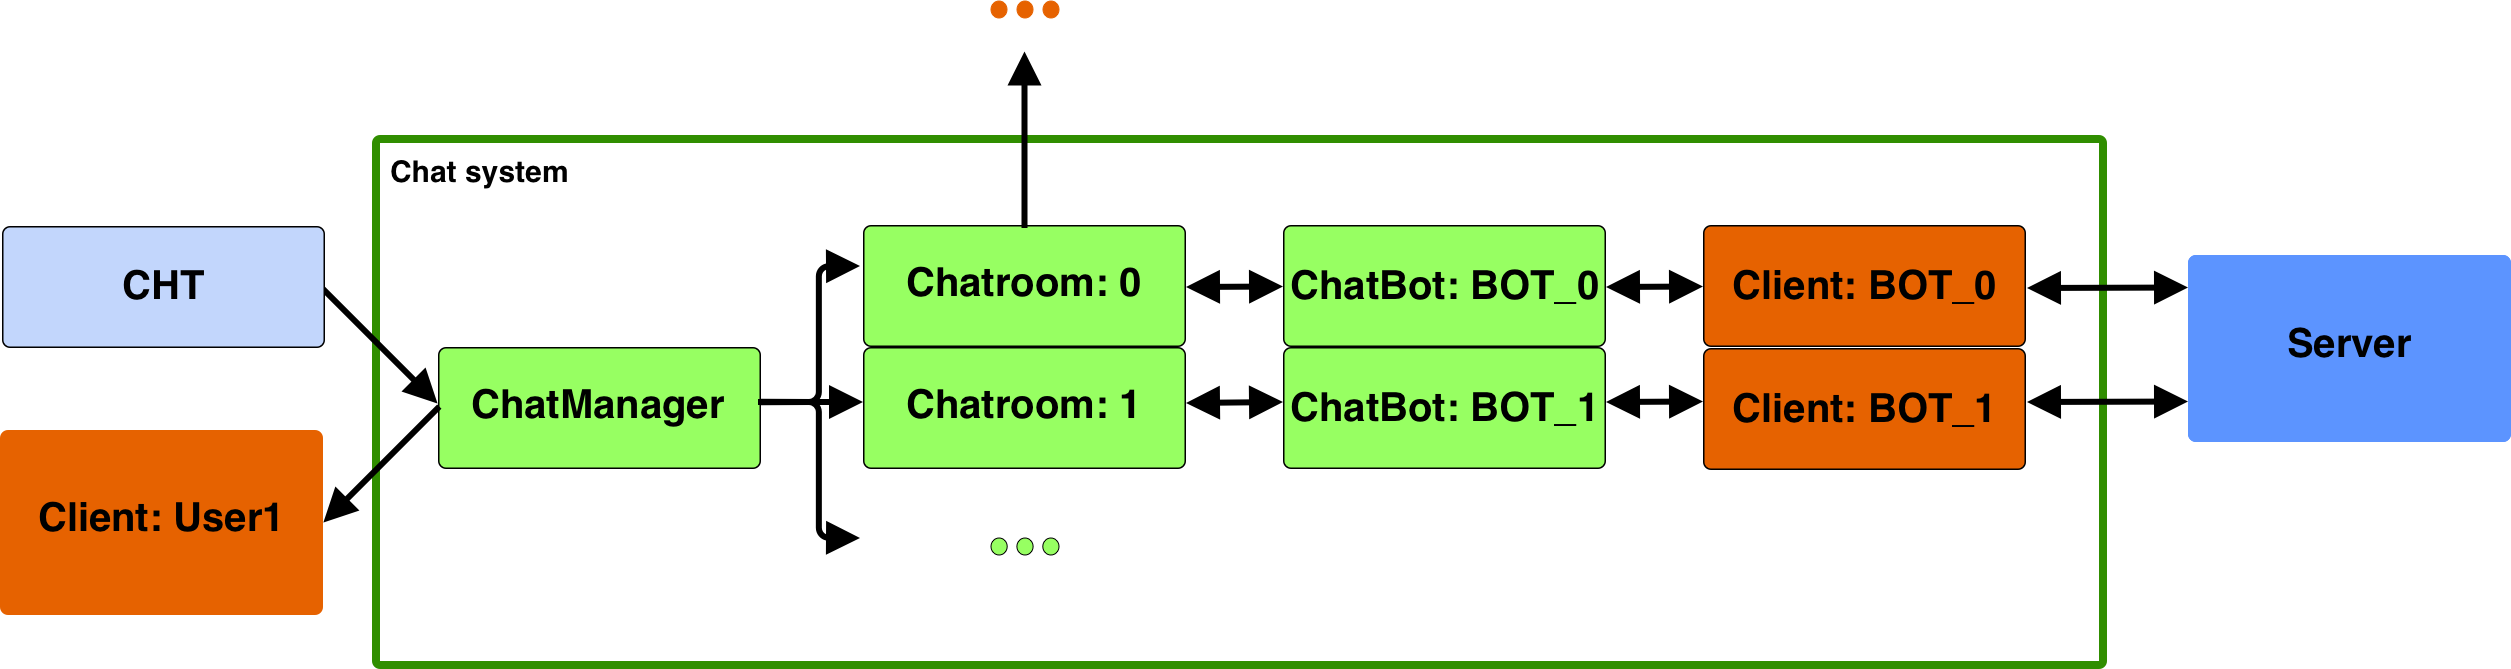
\includegraphics[width=\linewidth]{figures/chat/chat_arch.png}
	\caption{Chat system}
\end{figure}

\begin{figure}[h]
	\centering
	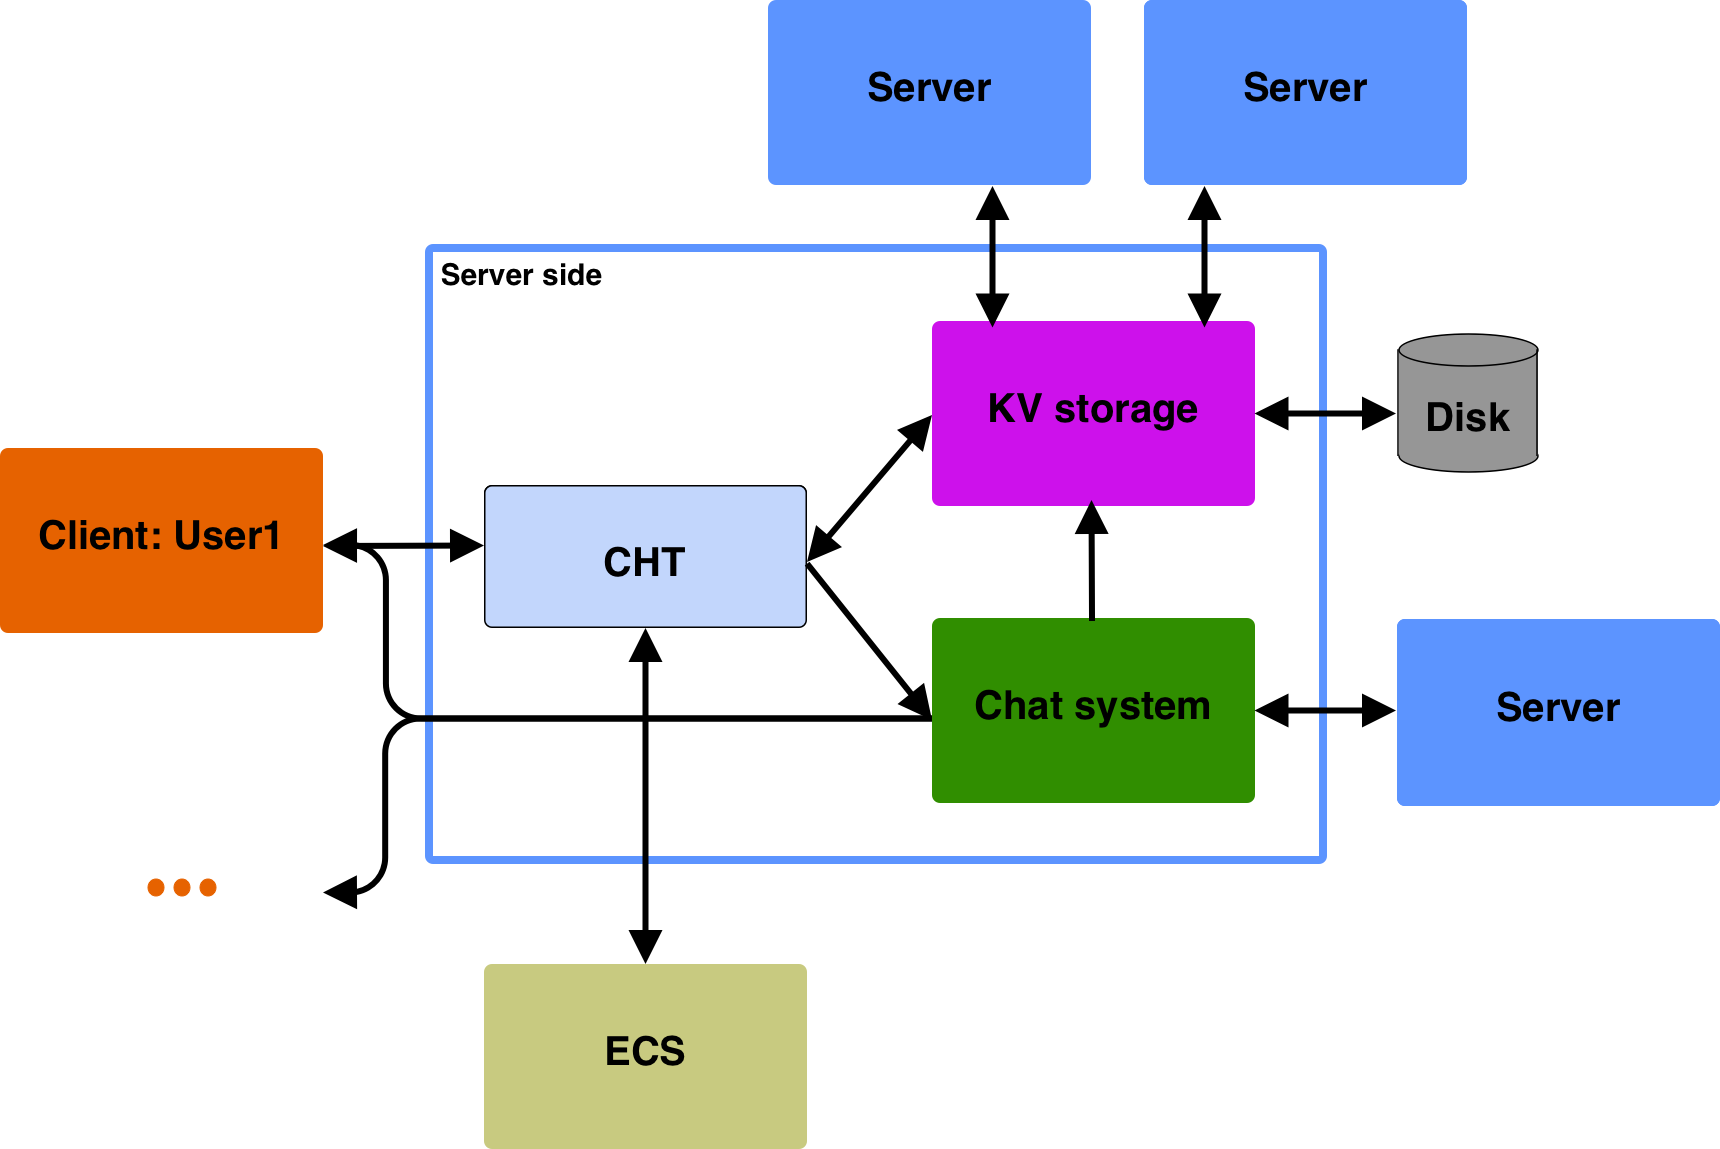
\includegraphics[width=\linewidth]{figures/chat/chat_full_arch.png}
	\caption{Server side architecture}
\end{figure}

addinitonals:

chat system:
All chat related requests get transferred by the CHT to the ChatManager. This has a list of Chatroom objects. When a client tries to connect to a chatroom, the ChatManager checks the list whether a chatroom with the provided chatID already exists or not. In the former case, 
if the chatroom is public, the client is granted access or, in case of a private chatroom, requested to enter a password. In the event of no chatroom found with the given chatID, the client is allowed to create the chatroom by specifying its type and providing a password, if a private chatroom is chosen. In order to increase security, the password gets hashed on the client side and only the hash of the password is stored at the server side and used for validation.


Each server owns a list containing the active chatrooms that it is responsible for. In order for a client to join one of those chatrooms is that it would first need to connect to that server, similar to the way storing key-value pair functions. The decision, to make chatrooms accessible only from one server has both its advantages and disadvantages. For one, it reduces the complexity of the system because otherwise servers would need a way to exchange updates regarding the active chatrooms and chat users whenever a user joins or leaves.

A problem with our implementation is that if the chatIDs are not equally distributed across all servers, which may occur due to the unpredictable nature of the hashing function, a single server could then be in charge of most chatrooms. This would cause that a server to be overloaded with requests and would lead to greater response times and, in the worst-case scenario, would result in a bottleneck for the whole system. In order to combat this issue, we limit the number of chatrooms belonging to one server to 15 and the number of users in a single chatroom to 30. This means a server is responsible for up to 450 chat users. These limits could also be easily changed depending on the intended use case of the system.

The biggest advantage of our decision is that it heavily reduces network traffic. Since all chatroom users are connected to the same server, that server can easily forward messages between them. Otherwise additional socket connections would have been required which would have both increased the load on the network and the overall complexity of the system.

Our idea for the chatting functionality was for it to be as lightweight as possible with clients entering and leaving chatrooms regularly.

To prevent heavy workload for a server, a chatroom has the maximum capacity of 30 people. The chatroom offers a communication platform for all the clients sharing the same chatroom. Every message sent by the clients have timestamps in order to keep on track with the flow of the messages for other clients. One message can contain maximum 200 characters.

When a client joins a chatroom, all the messages which sent until that time, will be visible to the latest joined client and all the members will be informed about who joined or left the chatroom. 


/*At the start of the connection, the CHT contacts the ECS in order to assign the client a unique username. After that the CHT interacts exclusively with KV storage and the chat system, depending on the command issued by the client.*/


Put and delete operations are fulfilled with the help of a chatbot. Most of the software systems include a chatbot in their system to work as a costumer service. Our intention by implementing a chatbot is to decrease the workload of the chatroom.